
\chapter{Embedding array computations}
\label{ch:accelerate}

\epigraph{At the beginning of a novel, a writer needs confidence, but after that
what's required is persistence. These traits sound similar. They aren't.
Confidence is what politicians, seducers and currency speculators have, but
persistence is a quality found in termites. It's the blind drive to keep on
working that persists after confidence breaks down.}%
{\textsc{---walter kirn}}


Starting with Fortran, array-based code has played a central role in
high-performance computing. Array-based programming has proved to be successful
not only on data-parallel (SIMD) hardware such as the CM-2, vector computers,
and modern graphics processing units (GPUs), but also on control parallel (MIMD)
hardware such as distributed memory, symmetric multiprocessor (SMP), and
multicore machines.

Recent work on stream fusion in the vector
library~\cite{Coutts:2007kp,Mainland:2013ez} and the parallel array library
Repa~\cite{Keller:2010er,Lippmeier:2011cd,Lippmeier:2012gx} have demonstrated
that purely functional array code in Haskell (1) can be competitive with the
performance of imperative array programs; and (2) lends itself to an efficient
parallel implementation on control-parallel multicore CPUs.

So far, less successful has been the use of purely functional array programs for
programming data-parallel SIMD hardware. This chapter describes the Accelerate
language, our purely functional language over regular, multidimensional arrays,
which has been designed to allow efficient execution on massively data-parallel
hardware such as GPUs.


\section{The Accelerate EDSL}
\label{sec:accelerate}

The current generation of graphical processing units are massively multicore
processors (\S\ref{sec:gpu_computing}). They are optimised for workloads with a
large degree of data parallelism (\S\ref{sec:data_parallelism}) and good
performance depends on highly idiomatic programs with low SIMD divergence and
regular memory-access patterns~\cite{NVIDIA:2012wf}. These unusual
characteristics of GPUs means that the development of applications that use the
graphics processors for general purpose computations (\S\ref{sec:gpu_computing})
is work intensive and requires a substantial degree of expert knowledge.

Accelerate is our approach to reducing the complexity of GPU programming: a
high-level, deeply embedded domain-specific language (\S\ref{sec:EDSLs}) of
array computations that captures appropriate GPGPU idioms in the form of
parameterised, \indexe{rank-polymorphic}~\cite{Keller:2010er}, collective
operations on arrays~\cite{Chakravarty:2011fr}. Our choice of operations was
informed by the \emph{scan-vector model}~\cite{Chatterjee:1990vj}, which is
suitable for a wide range of algorithms, and demonstrated that these operations
can be efficiently implemented on modern GPUs~\cite{Sengupta:2007tc}.

We regard Accelerate's collective array operations as algorithmic
skeletons~(\S\ref{sec:code_generation}) that capture appropriate GPU programming
idioms. The dynamic code generator instantiates CUDA implementations of these
skeletons~(\S\ref{sec:parallel_algorithms_in_cuda}) to implement embedded array
programs~(\S\ref{sec:instantiating_skeletons}). Dynamic code generation exploits
runtime information of the target hardware to optimise GPU code, and enables
on-the-fly generation of embedded array programs by the host
program~(\S\ref{sec:dynamic_compilation}). The evaluator minimises the overhead
of dynamic code generation by caching binaries of previously compiled skeleton
instantiations and by parallelising code generation, data
transfer~(\S\ref{sec:memory_management}), and GPU kernel loading, configuration,
and execution~(\S\ref{sec:executing_programs}).

To achieve performance competitive with hand-written
CUDA~\cite{McDonell:2013wi}, we implement two primary optimisation techniques:
sharing recovery~(\S\ref{sec:sharing_recovery}) tackles code explosion due to
the embedding in Haskell, while array
fusion~(\S\ref{sec:array_fusion}) eliminates superfluous
intermediate structures, which often arise due to the high-level nature of the
language. Both of these techniques are well known from other contexts, but they
present unique challenges for an embedded language compiled for execution on a
GPU.

\begin{figure}
    \centering
    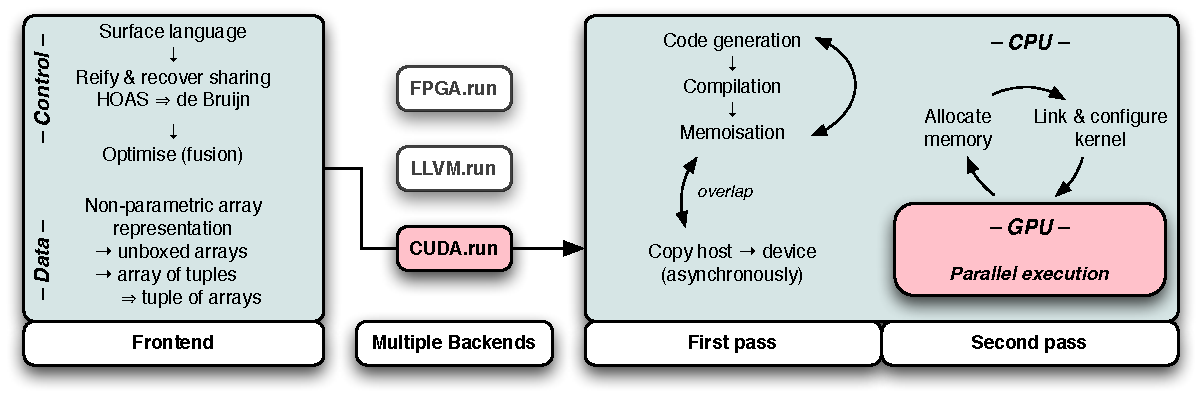
\includegraphics[width=\textwidth]{images/acc/outline-s}
    \caption[The overall structure of Accelerate]{The overall structure of
    Accelerate. It comprises a frontend and supports multiple backends that can
    target a variety of architectures.}
    \label{fig:outline}
\end{figure}

Figure~\ref{fig:outline} summarises the overall structure of Accelerate. It
comprises a frontend and support for multiple backends that can target a variety
of architectures. Here, we are only concerned with the CUDA generating GPU
backend, but the approach is amenable to targeting multicore CPU backends
exploiting SIMD instructions,\footnote{\url{https://github.com/AccelerateHS/accelerate-llvm}}
backends for OpenCL,\footnote{\url{https://github.com/AccelerateHS/accelerate-backend-kit/tree/master/icc-opencl}}\footnote{\url{https://github.com/HIPERFIT/accelerate-opencl/}}
and for reconfigurable hardware such as FPGAs. In the following, we briefly
introduce some features of the design and use of Accelerate.


\subsection{Computing a vector dot product}
\label{sec:computing_dotp}

Consider computing the dot product of two vectors, using standard Haskell lists:
%
\begin{lstlisting}[style=haskell]
dotp_list :: [Float] -> [Float] -> Float
dotp_list xs ys = foldl (+) 0 (zipWith (*) xs ys)
\end{lstlisting}
%
The two input vectors @xs@ and @ys@ are pointwise multiplied, and the resulting
list of products is summed, yielding the scalar result.

Using Accelerate, we implement this computation on arrays as follows:
%
\begin{lstlisting}[style=haskell]
dotp :: Vector Float -> Vector Float -> Acc (Scalar Float)                         -- (1)
dotp xs ys
    = let xs' = use xs                                                             -- (2)
          ys' = use ys
      in
      fold (+) 0 (zipWith (*) xs' ys')                                             -- (3)
\end{lstlisting}
%
Here, @fold@ and @zipWith@ are taken from the Accelerate library
@Data.Array.Accelerate@, rather than from the standard Haskell library
@Data.List@. The Accelerate code consumes two one dimensional arrays (@Vector@)
of values, and produces a single (@Scalar@) result as output. It differs from
the list version in three main respects:
%
\begin{enumerate}
    \item The result is an embedded Accelerate computation, indicated by the
        type constructor @Acc@. It will be evaluated in the \emph{target}
        language\index{language!target} of dynamically generated parallel code,
        rather than the \emph{meta} language\index{language!meta}, which is
        vanilla Haskell (\S\ref{sec:EDSLs}).

    \item We lift the two plain vectors @xs@ and @ys@ into @Acc@ terms with
        @use@. This makes the arrays available to the embedded computation
        (\S\ref{sec:arrays_on_the_host_and_device}).

    \item We use @fold@ instead of @foldl@.
\end{enumerate}
%
The first two points are artefacts of lifting the computation into an embedded
language (\S\ref{sec:EDSLs}), effectively delaying the computation. Concerning
the final point, the list traversal function @foldl@ guarantees a left-to-right
traversal of the elements, whereas @fold@ leaves the order in which the elements
are combined unspecified. This requires that the binary operator supplied to
@fold@ is associative and commutative,\footnote{Although floating-point
arithmetic is not strictly associative, it is common to accept the resulting
error in parallel applications.} but allows for an implementation using a
parallel tree reduction~\cite{Chatterjee:1990vj,Sengupta:2007tc}.


\subsection{Arrays, shapes, and indices}
\label{sec:arrays_shapes_and_indices}

Parallelism in Accelerate takes the form of collective operations such as
@zipWith@ on arrays of type @Array sh e@, where @sh@ is the \emph{shape} and @e@
the \emph{element type} of the array. Following the approach taken in
Repa~\cite{Keller:2010er}, we represent both the shapes and indices of an array
using an inductive notation of tuples as heterogeneous \emph{snoc} lists to
enable rank-polymorphic definitions of array functions.

As shown in Listing~\ref{lst:shapes_and_indices}, on both the type and value
level, the constructor @Z@ is used to represent the shape of a rank-0 array, and
the infix operator @(:.)@ is used to increase the rank by adding a new (innermost)
dimension to the right of the shape. Thus, a rank-3 index with components @x@,
@y@, and @z@, is written @(Z:.z:.y:.x)@ and has type @(Z:.Int:.Int:.Int)@, where
the component @x@ is innermost and varies most rapidly, while the component @z@
varies least rapidly.

\begin{lstlisting}[style=haskell_float
    ,label=lst:shapes_and_indices
    ,caption={Types of array shapes and indices}]
data Z            = Z                   -- rank zero
data tail :. head = tail :. head        -- increase rank by one

type DIM0 = Z                           -- synonynms for common array dimensionalities
type DIM1 = DIM0 :. Int
type DIM2 = DIM1 :. Int
type DIM3 = DIM2 :. Int
  -- and so on

type Array DIM0 e = Scalar e            -- synonynms for common array types
type Array DIM1 e = Vector e
\end{lstlisting}

Overall, an array of type @Array (Z:.Int:.Int) Float@ is a rank-2 array of
single precision floating-point numbers. Listing~\ref{lst:shapes_and_indices}
also defines synonyms for common array types: a singleton array of shape @DIM0@
represent a single scalar value, while an array of shape @DIM1@ represents a
vector, and so on. While it may appear that the explicit mentioning of @Int@ in
each dimension is redundant, we require indices over types other than @Int@ for
rank polymorphic functions, such as replicating an array into one or more
additional dimensions or slicing a lower-dimensional subarray out of a larger
array~\cite{Keller:2010er,Chakravarty:2011fr}.


\subsection{Arrays on the host and device}
\label{sec:arrays_on_the_host_and_device}

Accelerate is an \emph{embedded language} (\S\ref{sec:EDSLs}) that distinguishes
between vanilla Haskell arrays and arrays in the embedded language, as well as
computations on both flavours of arrays. Embedded array computations are
identified by types formed from the type constructor @Acc@, and must be
explicitly executed before taking effect. To make these arguments available to
the Accelerate computation they must be embedded with the @use@ function, which
is overloaded so that it can accept tuples of arrays:
%
\begin{lstlisting}[style=haskell]
use :: Arrays arrays => arrays -> Acc arrays
\end{lstlisting}
%
In the context of GPU programming, GPUs typically have their own
high-performance memory which is separate from the host CPU's main memory, and
data must be explicitly transferred to the GPU's memory before it can be used.
The distinction between regular arrays of type @Array sh e@ and arrays of the
embedded language @Acc (Array sh e)@ has the added benefit of differentiating
between arrays allocated in host memory and arrays allocated in GPU device
memory. Thus, @use@ also implies a host-to-device data transfer. See
section~\ref{sec:memory_management} for more information on how device memory is
managed. Similarly, expressions in @Acc@ are computations that are executed on
the device (the GPU), whereas regular Haskell code runs on the host (the CPU).


\subsection{Array computations versus scalar expressions}
\label{sec:array_computations_vs_scalar_expressions}

The signatures of the two operations @zipWith@ and @fold@, used in the
definition of @dotp@, are shown in Listing~\ref{lst:acc_operations}. These
operations are multidimensional variants of the corresponding list functions,
but with arrays wrapped in @Acc@. In addition to @Acc@, which marks embedded
array computations, we also have @Exp@, which marks \emph{embedded scalar}
computations: a term of type @Exp Int@ represents an embedded expression
yielding a value of type @Int@, and similarly @Exp Float -> Exp (Float,Float)@
characterises an embedded scalar function that takes an argument of type @Float@
and yields a pair of @Float@s as the result. As with computations embedded in
@Acc@, computations in @Exp@ are executed in the target language of GPU device
code.

\begin{lstlisting}[style=haskell_float,
    numbers=none,
    float=t,
    label={lst:acc_operations},
    caption={[Core Accelerate array operations] Summary of Accelerate's core
        collective array operations, omitting \code{Shape} and \code{Elt} class
        constraints for brevity. In addition, there are other flavours of folds
        and scans as well as segmented versions of these.}]
use         :: Array sh e -> Acc (Array sh e)                         %\rm embed an array%
unit        :: Exp e -> Acc (Scalar e)                                %\rm create singleton array%

reshape     :: Exp sh -> Acc (Array sh' e) -> Acc (Array sh e)        %\rm impose a new shape%

map         :: (Exp a -> Exp b) -> Acc (Array sh a)                   %\rm map a function over an array%
            -> Acc (Array sh b)
zipWith     :: (Exp a -> Exp b -> Exp c) -> Acc (Array sh a)          %\rm apply funciton to a\ldots%
            -> Acc (Array sh b) -> Acc (Array sh c)                   %\rm \ldots pair of arrays%

generate    :: Exp sh -> (Exp sh -> Exp a) -> Acc (Array sh a)        %\rm array from index mapping%

replicate   :: Slice slix                                             %\rm extend array across\ldots%
            => Exp slix -> Acc (Array (SliceShape slix) e)            %\rm \ldots new dimensions%
            -> Acc (Array (FullShape slix) e)
slice       :: Slice slix                                             %\rm remove existing dimensions%
            => Acc (Array (FullShape  slix) e) -> Exp slix
            -> Acc (Array (SliceShape slix) e)

fold        :: (Exp a -> Exp a -> Exp a) -> Exp a                     %\rm tree reduction along\ldots%
            -> Acc (Array (sh:.Int) a) -> Acc (Array sh a)            %\rm \ldots innermost dimension%
scan{l,r}   :: (Exp a -> Exp a -> Exp a) -> Exp a -> Acc (Vector a)   %\rm left-to-right or right-to-left\ldots%
            -> Acc (Vector a)                                         %\rm \ldots vector pre-scan%

backpermute :: Exp sh' -> (Exp sh' -> Exp sh) -> Acc (Array sh a)     %\rm backwards permutation%
            -> Acc (Array sh' e)
permute     :: (Exp a -> Exp a -> Exp a) -> Acc (Array sh' a)         %\rm forward permutation%
            -> (Exp sh -> Exp sh') -> Acc (Array sh a)
            -> Acc (Array sh' a)

stencil     :: Stencil sh a stencil => (stencil -> Exp b)             %\rm map a function with local\ldots%
            -> Boundary a -> Acc (Array sh a) -> Acc (Array sh b)     %\rm \ldots neighbourhood context%
\end{lstlisting}

Accelerate distinguishes the types of collective and scalar computations to
achieve a stratified language. Collective operations in @Acc@ comprise many
scalar computations in @Exp@ that are executed in parallel. However, scalar
computations \emph{can not} contain collective operations. This stratification
excludes \emph{nested, irregular} data parallelism statically --- instead,
Accelerate is restricted to \emph{flat data-parallelism} involving only regular,
multi-dimensional arrays.

Compared to regular Haskell, @Exp@ computations are rather limited in order to
meet the restrictions of what can be efficiently executed on GPUs\@. In
particular, we do not support recursion, and provide only a limited form of
explicit value iteration. Scalar expressions support Haskell's standard arithmetic
operations by overloading the standard type classes such as @Num@ and @Integaral@,
as well as bitwise operations from @Bits@. Although we can not overload
functions on @Bool@ in standard Haskell, we support equality and comparison
operators as well as logical connectives using the operators @(==*)@, @(/=*)@,
@(<*)@, \lstinline[style=inline,literate=]{(<=*)},      % don't turn into (≤*)
and so on. We also have conditional expressions in the form of @c ? (t, e)@,
which evaluates to @t@ if @c@ yields @True@, otherwise to @e@. There are also
scalar operations that take array valued arguments; namely, @arr!ix@ indexes an
array and @shape@ queries the extent of an array. The argument to these
operations is guaranteed to only be a previously let-bound variable, ensuring
that each invocation of the scalar function can not initiate additional
parallel work. Finally, we have tupling and projection, and auxiliary functions
for computing with indices.


\subsection{Computing an $n$-body gravitational simulation}
\label{sec:computing_nbody}

At a second example, consider simulating the Newtonian gravitational forces on a
set of massive bodies in 3D space, using a precise (but expensive) O($n^2$)
algorithm. We use the following type synonyms to represent bodies in the
simulation:
%
\begin{lstlisting}[style=haskell]
type Vec a      = (a, a, a)
type Position   = Vec Float
type Accel      = Vec Float

type Mass       = Float
type PointMass  = (Position, Mass)
\end{lstlisting}
%
@Vec@ is the type of 3-component vectors, which are used to store the $x$-,
$y$-, and $z$-components of the particle's position or acceleration in 3D space
along each dimension in @Position@ and @Accel@ respectively. A @PointMass@ is a
tuple containing the body's @Mass@ and @Position@.

In a data-parallel setting, the natural implementation first computes the forces
between every pair of bodies, before reducing the components applied to each
body using a multidimensional (segmented) reduction. In Accelerate, we can calculate
the acceleration each body experiences as it interacts with all other bodies in
the system as follows:
%
\begin{lstlisting}[style=haskell]
calcAccels :: Exp R -> Acc (Vector PointMass) -> Acc (Vector Accel)
calcAccels epsilon bodies
  = let n       = A.size bodies
        cols    = A.replicate (lift $ Z :. n :. All) bodies                        -- (1)
        rows    = A.replicate (lift $ Z :. All :. n) bodies
    in
    A.fold (.+.) (vec 0)                                                           -- (3)
      $ A.zipWith (accel epsilon) rows cols                                        -- (2)
\end{lstlisting}
%
\begin{enumerate}
\item @replicate@ expands the vector of @n@ bodies into an @n@$\times$@n@
    matrix, where we replicate the original elements of the source vector,
    represented by @All@, such that every element down the columns or along the
    rows of the matrix are identical, respectively. The operation @lift@ is used
    to push the shape constructors into the expression; that is, in this
    instance we have @lift :: (Z :. Exp Int :. All) -> Exp (Z :. Int :. All)@.

\item @zipWith@ calculates the interaction between each pair of particles by
    element wise combining the @n@$\times$@n@ matrices, which were replicated in
    opposite directions.
    % Since we replicated the source vector along the rows and columns, this
    % computes all $n^{2}$ interactions.

\item @fold@ reduces the result along the innermost dimension only, yielding a
    vector containing the sum of interactions for each particle between all
    others. The auxiliary function @(.+.)@ performs component-wise addition of
    the 3-vector.
\end{enumerate}

This is an example of using rank polymorphic operations in Accelerate. The
function @fold@ requires an argument array of at least rank-1 (such as a
matrix), and the result is computed by reducing the array along the innermost
dimension, reducing the rank of the array by one (in this case yielding a
vector). The functions @replicate@ and @slice@ are rank polymorphic as well, but
require more complex shape constraints that we characterise with the type family
@FullShape@ and @SliceShape@ that statically track changing array dimensions.
For details on the various forms of shape polymorphism,
see~\cite{Keller:2010er}. Overall, as shown in Listing~\ref{lst:acc_operations},
the collective operations of Accelerate are a multi-dimensional variant of those
underlying the scan-vector model~\cite{Chatterjee:1990vj,Sengupta:2007tc}.


\subsubsection{Computing gravitational potential}

We briefly explain how to compute the gravitational potential between a pair of
bodies. Given $n$ bodies with position $\mathbf{x}_i$ and velocity
$\mathbf{v}_i$ for $i \in [1,n]$ (bold face indicates a 3-component vector), the
force $\mathbf{f}_{ij}$ on a body $i$ is caused by its gravitational attraction
to body $j$ is given by:
%
\begin{equation*}
    \mathbf{f}_{ij}
      = G \frac{m_i m_j}{\left|\mathbf{r}_{ij}\right|^2}
        \cdot
        \frac{\mathbf{r}_{ij}}{\left|\mathbf{r}_{ij}\right|}
\end{equation*}
%
where $m_i$ and $m_j$ are the masses of the bodies, $\mathbf{r}_{ij} =
\mathbf{x}_j - \mathbf{x}_i$ is the vector from body $i$ to body $j$, and $G$ is
the gravitational constant. The factor on the left represents the
\emph{magnitude} of the acceleration, and is proportional to the product of the
masses and diminishes as the square of the separation of the masses. The right
factor is the \emph{direction} of the force, and is the unit vector from $i$ in
the direction of $j$.

The total force $\mathbf{F}_i$ on a body $i$ due to its interactions with the
other bodies is thus:
%
\begin{equation*}
    \mathbf{F}_i
      = \sum_{\substack{1 \le j \le n\\j \ne i}} \mathbf{f}_{ij}
      = G m_i \cdot \sum_{\substack{1 \le j \le n\\j \ne i}}
            \frac{m_j \mathbf{r}_{ij}}{\left|\mathbf{r}_{ij}\right|^3}
\end{equation*}
%
Note that as the bodies approach each other, the force between them grows
without bound, which is undesirable for numerical simulations. In astrophysical
simulation, collisions between bodies are generally precluded, which is
reasonable if the bodies represent galaxies that may pass through each other. A
\emph{softening factor} $\epsilon^2 > 0$ is added, which models the interaction
of two Plummer point masses~\cite{Aarseth:2003uz,Dyer:1993bk}. In effect,
softening limits the magnitude of forces between bodies. The denominator is
rewritten as follows:
%
\begin{equation*}
    \mathbf{F}_i \approx G m_i \cdot \sum_{1 \le j \le n}
        \frac{m_j \mathbf{r}_{ij}}
             {\left( \left|\mathbf{r}_{ij}\right| + \epsilon^2 \right)^{\sfrac{3}{2}}}
\end{equation*}
%
The condition $j \ne i$ is no longer needed, because $\mathbf{f}_{ii} = 0$ when
$\epsilon^2 > 0$.

Finally, the acceleration experienced by a body is $\mathbf{a}_i =
\mathbf{F}_i/m_i$, and we can now present the Accelerate routine to compute the
acceleration between two bodies.
%
%\begin{equation*}
%    \mathbf{a}_i \approx
%    G \sum_{1 \le j \le n}
%      \frac{m_j \mathbf{r}_{ij}}
%           {\left( \left|\mathbf{r}_{ij}\right|^2 + \epsilon^2 \right)^{\sfrac{3}{2}}}
%\end{equation*}
%
%
\begin{lstlisting}[style=haskell]
accel :: Exp R -> Exp PointMass -> Exp PointMass -> Exp Accel
accel epsilon pmi pmj = (mj * invr3) *. r
  where
    mj          = massOfPointMass pmj
    r           = positionOfPointMass pmj .-. positionOfPointMass pmi
    rsqr        = dot r r + epsilon * epsilon
    invr        = 1 / sqrt rsqr
    invr3       = invr * invr * invr
\end{lstlisting}
%
Here the functions @positionOfPointMass@ and @massOfPointMass@ extract each
component of the @PointMass@, respectively. The function @(.-.)@ is
component-wise subtraction applied to the 3-vector, and @(*.)@ multiplies each
component of a 3-vector by a scalar value.


\subsection{Non-parametric array representation}

In order to make arrays available for use in embedded computations, we have the
function @use@ (\S\ref{sec:arrays_on_the_host_and_device}). For a single array,
it has the type:
%
\begin{lstlisting}[style=haskell]
use :: (Shape sh, Elt e) => Array sh e -> Acc (Array sh e)
\end{lstlisting}
%
The type classes @Shape@ and @Elt@ characterise the types that may be used as
array indices and array elements respectively. We discussed the nature of array
indices in section~\ref{sec:arrays_shapes_and_indices}. The @Elt@ class
characterises the types of values that can be used as array elements, and hence
appear in scalar Accelerate expressions. The supported @Elt@ types are signed \&
unsigned integers (8, 16, 32, and 64-bit wide), floating point numbers (single
\& double precision), as well as @Char@, @Bool@, and array indices formed from
@Z@ and @(:.)@. Furthermore, there are tuples of all of those, including nested
tuples, as was seen in the $n$-body example~(\S\ref{sec:computing_nbody}).

Accelerate arrays of primitive type, such as @Int@ and @Float@, are easily
represented as arrays of the corresponding integral and floating point types.
More interesting is the case of arrays of tuples, where we use a non-parametric
array representation so that arrays of tuples are represented in memory as a
tuple of arrays, one array for each primitive type in the structure. By virtue
of this representation, Accelerate is able to make optimal use of the available
memory bandwidth. See section~\ref{sec:representing_tuples} for details.

Moreover, consider the following types:
%
\begin{lstlisting}[style=haskell]
data Point = P Int Int

point :: Exp Point
sh    :: Exp (Z :. Int :. Int)
tup   :: Exp (Int, Int)
\end{lstlisting}
%
The salient feature of each type is that it carries two integers, albeit each
wrapped in different constructors. We call this the
\emph{surface}\index{type!surface} type of a term. However, an Accelerate
backend implementation should not need to know about the surface type
representation. Indeed, we do not want to have to extend the backend to support
every new user-defined type such as @Point@. The @Elt@ class tells us how to
convert between the surface type of an expression that a user programs in, into
the \emph{representation} type\index{type!representation} that an implementation
stores and computes data in. We use a type
family~\cite{Chakravarty:2005dx,Schrijvers:2008ir} of nested tuples to represent
types as heterogenous snoc-lists of primitive types:
%
\begin{lstlisting}[style=haskell]
type family EltRepr a :: *
type instance EltRepr ()        = ()
type instance EltRepr Int       = ((), Int)
type instance EltRepr Float     = ((), Float)
type instance EltRepr (a, b)    = (EltRepr a, EltRepr' b)
type instance EltRepr (a, b, c) = (EltRepr (a, b), EltRepr' c)
  -- and so on\ldots
\end{lstlisting}
%
Here @EltRepr'@ is similar, except that we use a flattened representation at the
leaves in order to avoid overly nested pairs; that is, primitive types are
represented as @EltRepr' Int = Int@. Arrays of tuples have a similar mapping
into a nested tuple of arrays, defined by the @Arrays@ class.


\subsection{Richly typed terms}
\label{sec:richly_typed_terms}

%\marginnote{tk: this bit is very implementation-y}
As a deeply embedded language, the operations of both the array and scalar
sub-language do not directly issue computations; instead, they build term trees
to represent embedded computations (\S\ref{sec:EDSLs}). The terms in the surface
language use \indexe{higher-order abstract syntax} (HOAS) to embed
function-valued scalar expressions as well as type class overloading to reflect
arithmetic expressions. For example, the body of the @dotp@ function
% @fold (+) 0 (zipWith (*) xs' ys')@
is translated into:\footnote{The subterms to \footcode{add} and \footcode{mul}
here are inline into the \footcode{Fold} and \code{ZipWith} terms respectively,
we only use a \footcode{where}-clause to improve readability.}
%
\begin{lstlisting}[style=haskell]
Fold add (Const 0) (ZipWith mul xs' ys')
  where
    add = \x y -> PrimAdd (FloatingNumType (TypeFloat FloatingDict))               -- (1)
                  `PrimApp`
                  Tuple (NilTup `SnocTup` x
                                `SnocTup` y)
    mul = -- as \emph{\texttt{add}}, but using \emph{\texttt{PrimMul}} ...
\end{lstlisting}
%
This is very much like the approach taken by \citet{Elliott:2004hh},
\citet{Gill:2011wy}, and \citet{Mainland:2010vj}. The difference is that in our
approach we use GADTs~\cite{Jones:2006eh} and type
families~\cite{Chakravarty:2005dx,Schrijvers:2008ir} to preserve the embedded
program's type information in the term tree (1), and use type-preserving
transformations in the front end (\S\ref{sec:manipulating_embedded_programs}).

The HOAS representation, while convenient for a human reader, is awkward
for program transformations as it complicates looking under lambdas; i.e.
inspecting and manipulating the bodies of function abstractions. After the
frontend reifies the embedded program written in HOAS, it recovers sharing
(\S\ref{sec:sharing_recovery}) while converting the HOAS representation into a
\emph{nameless} representation using \emph{typed de Bruijn indices}\index{de
Bruijn} in the style of~\citet{Altenkirch:2003kz}. The type preserving
conversion from HOAS to a nameless de Bruijn representation using
GADTs~\cite{Chakravarty:2009uo} was simultaneously discovered
by~\citet{Atkey:2009dj}.

Overall, the nameless form of @dotp@ is:
%
\begin{lstlisting}[style=haskell]
Fold add (Const 0) (ZipWith mul xs' ys')
  where
    add = Lam (Lam (Body (
        PrimAdd (FloatingNumType (TypeFloat FloatingDict))
                `PrimApp`
                Tuple (NilTup `SnocTup` (Var (SuccIdx ZeroIdx))
                              `SnocTup` (Var ZeroIdx)))))
    mul = -- as \emph{\texttt{add}}, but using \emph{\texttt{PrimMul}} ...
\end{lstlisting}
%
The @Lam@ constructor introduces nameless abstractions and @Var@ wraps a de
Bruijn index. At this point, the program is further optimised by the frontend,
for example by applying the fusion transformation~(\S\ref{sec:array_fusion}).

Finally, we represent the environment as a heterogenous snoc-list, encoded on
the type level as nested pairs and building this list on the value level with
the two constructors:
%
\begin{lstlisting}[style=haskell]
data Val env where
    Empty :: Val ()
    Push  :: Val env -> t -> Val (env, t)
\end{lstlisting}
%
A nameless \indext{de Bruijn} index projects out a specific type from the
environment:
%
\begin{lstlisting}[style=haskell]
data Idx env t where                                -- an index is either\ldots
    ZeroIdx ::              Idx (env, t) t          -- \ldots at the top of the stack, or\ldots
    SuccIdx :: Idx env t -> Idx (env, s) t          -- \ldots under some junk
\end{lstlisting}
%
Indices have type @Idx env t@, where the type @env@ keeps track of what
variables are in scope using the same encoding of nested tuples used by the
environment, while @t@ represents the type of a distinguished element in this
list. At the value level, @Idx@ encodes the index of that element in the list.

As terms are pushed into the environment, the type of the new term becomes
wrapped in the type of the environment; i.e.\ @t@ is existentially quantified in
@Push@. Our de Bruijn indices recover the wrapped type of individual elements by
projecting the index through the environment:
%
\begin{lstlisting}[style=haskell]
prj :: Idx env t -> Val env -> t
prj ZeroIdx       (Push _   v) = v
prj (SuccIdx idx) (Push val _) = prj idx val
prj _             _            = error "inconsistent valuation"
\end{lstlisting}

% \marginnote{tk: use Let/Alet constructor as further example?}
Overall, this is an example of using nested datatypes and polymorphic recursion
to precisely enforce constraints and invariants in the type of a term; in this
case the type and scope of bound variables. Since an embedded Accelerate program is
constructed and evaluated at program \emph{runtime}, encoding properties in the
type means that these invariants are checked at \emph{compile} time, reducing
the number of possible runtime errors in type-correct programs.


\section{Manipulating embedded programs}
\label{sec:manipulating_embedded_programs}

The Accelerate core language is richly typed, maintaining full type information
of the embedded language in the term tree. In order to apply transformations to
these terms while maintaining the correctness of the program as encoded in its
type, we require methods to manipulate these richly typed terms in a type- and
scope-preserving manner. This section covers several technique for manipulating
the embedded Accelerate programs, that are required to implement the
optimisations discussed in the following chapter.


\subsection{Typed equality}
\label{sec:equality}

If we want to test whether two Accelerate terms are equal --- for example, to
determine whether the subexpressions can be shared --- we immediately run into
the problem that terms in the core Accelerate language are existentially typed.
That is, how should we implement:
%
\begin{lstlisting}[style=haskell]
Exp s == Exp t = ??
\end{lstlisting}
%
There is no reason that @s@ and @t@ should be expressions of the same
type. In some instances we might not care, and as such can define standard
heterogeneous equality:
%
\begin{lstlisting}[style=haskell]
instance Eq (PreOpenExp acc env aenv t) where
    (==) = heq
    where heq :: PreOpenExp acc env aenv a -> PreOpenExp acc env aenv b -> Bool
          heq = ...
\end{lstlisting}
%
where we do not care about the result type of each expression, and only require
that the environment type, re size, of free scalar and array variables are the
same so that we can test equality of \indext{de Bruijn} indices.

However, we often \emph{do} care about the specific types of our existentially
quantified terms. Consider the case of defining equality for let-bindings.
The Accelerate scalar language defines let-bindings of the embedded program as a
constructor of a GADT~\cite{Jones:2006eh}, whose type tracks the type and scope
of the bound term (\S\ref{sec:richly_typed_terms}):
%
\begin{lstlisting}[style=haskell]
data PreOpenExp acc env aenv t where
    Let :: (Elt bnd_t, Elt body_t)                      -- Local binding of a scalar expression
        => PreOpenExp acc env          aenv bnd_t       -- bound term
        -> PreOpenExp acc (env, bnd_t) aenv body_t      -- body/scope of binding
        -> PreOpenExp acc env          aenv body_t

    -- other language constructs\ldots
\end{lstlisting}
%
To apply @heq@ to the body expression, we need to know something about
the type of the bound terms to ensure that the scalar environments are the same,
namely \lstinline[style=inline,mathescape]{a $\sim$ bnd_t $\sim$ b}.%
\footnote{Alternatively we can use \footcode{Data.Typeable.gcast} to provide a
type-safe cast, but this quickly becomes unwieldy and is a little
unsatisfactory.} To do this we must equip terms with a runtime witness to the
existentially quantified type. Our reified dictionaries will allow us to do
exactly this, so we can define heterogeneous equality for reified dictionaries:
%
\begin{lstlisting}[style=haskell]
heqIntegralType :: IntegralType s -> IntegralType t -> Bool
heqIntegralType (TypeInt _)  (TypeInt _)  = True
heqIntegralType (TypeWord _) (TypeWord _) = True
  ...
heqIntegralType _            _            = False
\end{lstlisting}
%
However, doing this is perfectly useless as it only gives us a value of type
@Bool@, with no idea what that value means or to what its truth might
entitle us. The type checker does not gain any useful knowledge about the types
the dictionaries @a@ and @b@ witness simply by knowing that
@heqIntegralType a b = True@. A boolean is a bit uninformative.

Instead, we can write essentially the same test, but in the positive case
deliver some \emph{evidence} that the types are equal:
%
\begin{lstlisting}[style=haskell]
data s :=: t where
    REFL :: s :=: s

matchIntegralType :: IntegralType s -> IntegralType t -> Maybe (s :=: t)
matchIntegralType (TypeInt _)  (TypeInt _)  = Just REFL
matchIntegralType (TypeWord _) (TypeWord _) = Just REFL
  ...
matchIntegralType _            _            = Nothing
\end{lstlisting}
%
Matching on @Just REFL@ will inject the knowledge into the type
checker that the types @s@ and @t@ are the same. Now with our
evidence-producing heterogeneous equality test for reified dictionary families,
we can compare two terms and gain type-level knowledge when they witness the
same value-level types. These witnesses for existentially quantified types then
allow us to test for equality \emph{homogeneously}, ensuring that positive
results from singleton tests give the bonus of unifying types for other tests:
%
\begin{lstlisting}[style=haskell]
matchPreOpenExp
    :: PreOpenExp acc env aenv s
    -> PreOpenExp acc env aenv t
    -> Maybe (s :=: t)
matchPreOpenExp (Let x1 e1) (Let x2 e2)
  | Just REFL <- matchOpenExp x1 x2     -- if the bound expressions match
  , Just REFL <- matchOpenExp e1 e2     -- then the environment of the body term will also match
  = Just REFL

matchPreOpenExp ...
\end{lstlisting}


\subsubsection{Congruence}

As we are interested in the facility of matching terms for the purposes of
optimisations such as common subexpression elimination (\S\ref{sec:cse}), it is
beneficial to define not equality but instead \indexe{congruence} of terms. Two
nodes are considered congruent if the nodes they label are constants and the
constants are equal; or they have the same operator and the operands are
congruent. The crux of the latter condition refers to commutative relations,
such as scalar addition, where an operator yields the same result when the order
of the operands are reversed. When checking equality of primitive applications,
we discriminate binary functions whose arguments commute, and return those
arguments in a stable ordering by comparing a hash of each of the sub-terms.
%
\begin{lstlisting}[style=haskell]
commutes
    :: PrimFun (a -> r)
    -> PreOpenExp acc env aenv a
    -> Maybe (PreOpenExp acc env aenv a)
commutes f x = case f of
  PrimAdd _     -> Just (swizzle x)
    ...         -> Nothing
  where
    swizzle :: PreOpenExp acc env aenv (a,a) -> PreOpenExp acc env aenv (a,a)
    swizzle exp
      | Tuple (NilTup `SnocTup` a `SnocTup` b) <- exp
      , hashPreOpenExp a > hashPreOpenExp b     = Tuple (NilTup `SnocTup` b `SnocTup` a)
      | otherwise                               = exp
\end{lstlisting}


\subsection{Simultaneous substitution}
\label{sec:substitution}

In order to do things like renaming and substitution we require a value-level
substitution algorithm for the richly typed terms. The implementation follows
the method of \citet{McBride:2006up,McBride:2005jv}, where it is seen that
renaming and substitution are both instances of a \emph{single} traversal
operation, pushing functions from variables to ``stuff'' through terms, for a
suitable notion of stuff.
%
The trick is to push a \emph{type-preserving} but \emph{environment changing}
operation structurally through terms:
%
\begin{lstlisting}[style=haskell]
v :: forall t'. Idx env t' -> f env' t'
\end{lstlisting}

Where the operation differs is in the image of variables: renaming maps
variables to variables and substitution maps variables to terms. We then lift
this to an operation which traverses terms, with appropriate lifting to push
under a lambda, and rebuilding the term after applying @v@ to the
variables:
%
\begin{lstlisting}[style=haskell]
rebuild :: Syntactic f
        => (forall t'. Idx env t' -> f env' t')
        -> Term env  t
        -> Term env' t
\end{lstlisting}

The @Syntactic@ class\footnote{Since Accelerate is a stratified language
there are separate implementations of this toolkit on syntactic elements for the
scalar and collective operations, but the details are identical. The discussion
uses the generic \footcode{Term} to mean either of these operations.} tells us
everything we need to know about @f@ --- our notion of ``stuff'' --- in
order to rebuild terms: a mapping in from variables, a mapping out to terms, and
a weakening map which extends the context. Renaming will instantiate @f@
with @Idx@, whereas for substitutions we may choose @Term@ instead.
%
\begin{lstlisting}[style=haskell]
class Syntactic f where
    varIn   :: Idx env t -> f env t             -- variables embed in f
    termOut :: f env t   -> Term env t          -- f embeds in terms
    weaken  :: f env t   -> f (env, s) t        -- f allows weakening

instance Syntactic Idx
instance Syntactic Term
\end{lstlisting}

A key component of this toolkit, \indexe{weakening} describes an operation we
usually take for granted: every time we learn a new word, old sentences still
make sense; if a conclusion is justified by a hypothesis, it is still justified
if we add more hypotheses; a term remains in scope if we bind new (fresh)
variables. Weakening is the process of shifting things from one scope to a
larger scope in which new things have become meaningful, but no old things have
vanished. When we use a named representation (or HOAS\index{higher-order
abstract syntax}\index{HOAS|see{higher-order abstract syntax}}) we get weakening
for free, but in the de Bruijn\index{de Bruijn} representation weakening takes
work: we need to shift all the variable references to make room for new
bindings. To do this we need to explain how to shift the @v@ operation into
an extended environment; saying what to do with the new variable and how to
account for it on the output side.
%
\begin{lstlisting}[style=haskell]
shift :: Syntactic f
      => (forall t'. Idx env t' -> f env' t')
      -> Idx (env,  s) t
      -> f   (env', s) t
\end{lstlisting}
%
Overall, the crucial functionality of simultaneous substitution is to propagate
a class of operations on variables closed under shifting, which is what
@Syntactic@ and @rebuild@ offer.


\subsection{Inlining}
\label{sec:inlining}

\begin{lstlisting}[style=haskell_float
    ,label=lst:inlining
    ,caption={A simultaneous substitution to inline terms}]
subTop :: Term env s -> Idx (env, s) t -> Term env t
subTop s ZeroIdx      = s
subTop _ (SuccIdx ix) = Var ix

inline :: Term (env, s) t -> Term env s -> Term env t
inline body bnd = rebuild (subTop bnd) body
\end{lstlisting}

The final question, then, is how to write the function @v@ which we push
through terms, as the type @forall t'@ could be anything. After all, what
is the point of having a simultaneous substitution algorithm if we can't
specialise it to one-at-a-time substitution.

The function @subTop@ in Listing~\ref{lst:inlining} takes a replacement for the
top variable and returns a simultaneous substitution which eliminates @ZeroIdx@.
If we have a term with one free variable, we can use this to replace that
variable with a term. That is, @inline@ a term into all use sites of the free
variable.

The demonic $\forall$ --- which is to say that the quantifier is in a position
which gives us obligation, not opportunity --- of the operator @v@ forces
us to respect type: when pattern matching detects the variable we care about,
happily we discover that it has the type we must respect. The demon is not so
free to mess with us as one might at first fear.

% Typing rules; each rule types the general usage of a symbol, below the
% line, in terms of the parameters above the line.??

\subsection{Function composition}
\label{sec:function_composition}

The equivalent of unary function composition @(.)@ on terms can be
defined in a similar manner. A function @(a -> b)@ is equivalent to a
@Term@ of type @b@ and free variable @a@. Similar to inlining, we
replace an expression that uses the top variable with one that uses another,
remembering to bind the result of the first expression so that it can be reused
in the second without duplication.

\begin{lstlisting}[style=haskell_float
    ,label=lst:function_composition
    ,caption={A simultaneous substitution to compose unary function terms}]
dot :: Term (env, b) c -> Term (env, a) b -> Term (env, a) c
dot f g = Let g (rebuild split f)
  where
    split :: Idx (env, b) c -> Term ((env, a), b) c
    split ZeroIdx      = Var ZeroIdx
    split (SuccIdx ix) = Var (SuccIdx (SuccIdx ix))

compose :: Fun env (b -> c) -> Fun env (a -> b) -> Fun env (a -> c)
compose (Lam (Body f)) (Lam (Body g)) = Lam (Body (f `dot` g))
compose _              _              = error "compose: impossible case"
\end{lstlisting}

Note the type of @split@ in Listing~\ref{lst:function_composition}, which
creates space in the environment at the second index (@SuccIdx ZeroIdx@) for the
free variable @a@ to appear in the resultant @Term@, as the first index will be
bound to the result of the first expression @g@.

The function @compose@ finally lifts this to function terms by unwrapping the
lambda abstractions. Annoyingly, GHC's type checker can not determine that the
function type prohibits any valid term except those with a single lambda, so we
need a second catch-all case to suppress a compilation warning. In the remainder
of the text, we elide the impossible cases for brevity.


\subsection{Environment manipulation}
\label{sec:environment_manipulation}

As part of the fusion transformation of recasting terms we often need to lift
array valued inputs to be let-bound at higher points to avoid work duplication,
but at the same time we can not immediately add these bindings to the output
term because they will interfere with further fusion steps. We need to collect
these extra bindings separately from the main term, and add them to the output
term at some later point. Furthermore, we must ensure we correctly track the
types of the environments between the fused terms and the collected
let-bindings.

Listing~\ref{lst:Extend} defines a heterogeneous snoc-list of array terms that
witnesses how an array environment is extended by the application of these
operations.
%
\begin{lstlisting}[
    style=haskell_float,
    label={lst:Extend},
    caption={Extending an array environment}]
data Extend acc aenv aenv' where
    BaseEnv :: Extend acc aenv aenv
    PushEnv :: Arrays a
            => Extend     acc aenv aenv'
            -> PreOpenAcc acc      aenv' a
            -> Extend     acc aenv (aenv', a)
\end{lstlisting}
%
In the style of the \indext{de Bruijn} indices used for projecting environment
variables (\S\ref{sec:richly_typed_terms}), @Extend@ uses an inductive notion of
tuples as heterogeneous \emph{snoc} lists. In contrast to environment indices,
the base case does not refer to an empty environment, but instead the
environment @aenv@ which we are extending. This witnesses how to construct an
extended environment @aenv'@ by bringing new terms into scope, one at a time.
%
\begin{lstlisting}[style=haskell]
bind :: Arrays a
     => Extend     acc aenv aenv'
     -> PreOpenAcc acc      aenv' a
     -> PreOpenAcc acc aenv       a
bind BaseEnv         = id
bind (PushEnv env a) = bind env . Alet (inject a) . inject
\end{lstlisting}
%
The auxiliary function @inject :: PreOpenAcc acc aenv a -> acc aenv a@ completes
the knot tying trick (\S\ref{sec:knot_tying}) to complete the definition of each
of the array terms.


\subsubsection{Sinking}
\label{sec:sinking}

\begin{lstlisting}[
    style=haskell_float,
    label=lst:sinking,
    caption={Sinking terms to a larger environment}]
type env :> env' = forall t'. Idx env t' -> Idx env' t'

class Sink f where
    weaken :: env :> env' -> f env t -> f env' t

sink :: Sink f => Extend acc env env' -> f env t -> f env' t
sink env = weaken (k env)
  where
    k :: Extend acc env env' -> Idx env t -> Idx env' t
    k BaseEnv       = id
    k (PushEnv e _) = SuccIdx . k e
\end{lstlisting}

We define \emph{sinking} as the operation of shifting a term from one (array)
environment into another, where new things have come into scope according to
some witness, and no old things have disappeared.

Listing~\ref{lst:sinking} generalises @weaken@ from
section~\ref{sec:substitution} to increase the environment of an object @f@
based on some function on indices rather than shifting by a single de Bruijn
index. Thus we only need to traverse a term once no matter how many positions
the variable indices shift by. Using @sink@, we can weaken terms based on the
witness provided by @Extend@.



\section{Related work}

Conal's early work (vertigo), Nikola, Obsidian.


\section{Discussion}

This chapter has covered the design of our Haskell-based purely functional
embedded language, which can express a wide range of programs over regular
multidimensional arrays. We have also discussed methods for the type safe
representation of programs, and several base techniques for type preserving
manipulation of those programs.

The next chapter covers my implementation of the CUDA based Accelerate backend
which executes Accelerate programs on massively parallel GPUs. The next chapter
also covers issues such as caching, which must be considered in order to ensure
that the embedded language exhibits performance competitive to traditional
offline compiled languages.

